%%%%%%%%%%%%%% 25/02/2020 %%%%%%%%%%%%%%%% 
\subsection*{\textbf{25/02/2020}}
\subsubsection*{Days aims}
\begin{itemize}
    \item Finalize cuts to be made on $Z \rightarrow ee$ and $Z \rightarrow \mu\mu$
\end{itemize}

\subsubsection*{Day Summary}
\begin{itemize}
    \item Investigated background contributions to change in azimuthal angle.
    \item Began treatment of ee and mumu decays as separate processes, calculating cross sections for each.
    \item Initial cuts made for pt and cross sections calculated.
  
\end{itemize}


%%%%%%%%%%%%% 9:00 %%%%%%%%%%%%%
\subsubsection*{09:00 - Lead DG}
Start by comparing the difference in azimuthal angle of the two leptons being produced.
\\
Cuts used in Fig.\ref{fig:Zee-Stack_delta-phi_(min-cuts_2lep=ll)_25-02-21}
\begin{lstlisting}
    lepCut ="(" + "(lep_charge[0] != lep_charge[1]) && (lep_type[0]==11 && lep_type[1]==11) && lep_n==2" + ")"
    
    t.SetAlias("inv_mass_Zll","sqrt(2*lep_pt[0]*lep_pt[1]*(cosh(lep_eta[0]-lep_eta[1])-cos(lep_phi[0]-lep_phi[1])))")
    t.Draw("abs(lep_phi[0] - lep_phi[1]) >> h_lep_delta_phi(100,0,6.3)", weighting + "*" + lepCut)
\end{lstlisting}

\begin{figure}[h!]
    \centering
    \begin{minipage}{0.5\textwidth}
        \centering
        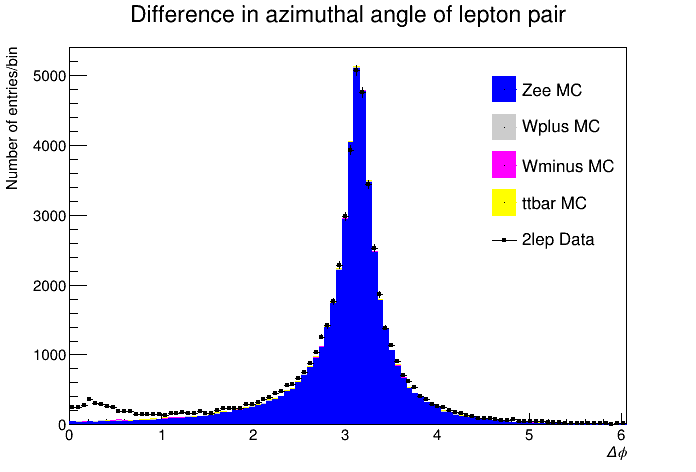
\includegraphics[width=\linewidth]{plots/25-02-2021/Zee-Stack_delta-phi_(min-cuts_2lep=ee)_25-02-21_09-25.png}
        (A)
    \end{minipage}\hfill
    \begin{minipage}{0.5\textwidth}
        \centering
        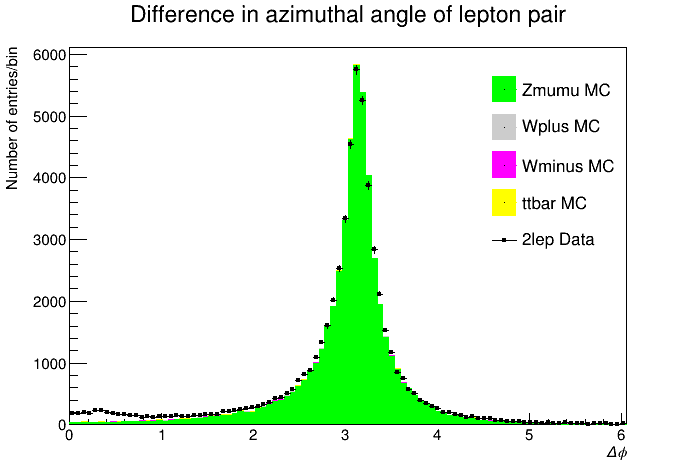
\includegraphics[width=\linewidth]{plots/25-02-2021/Zmumu-Stack_delta-phi_(min-cuts_2lep=mumu)_25-02-21_09-38.png}
        (B)
    \end{minipage}
    \caption{(A) Difference in azimuthal angle of ee pair produced. (B) Difference in azimuthal angle of $\mu\mu$ pair produced.  Cuts: }
    \label{fig:Zee-Stack_delta-phi_(min-cuts_2lep=ll)_25-02-21}
\end{figure}

\begin{lstlisting}
    lepCut ="(" + "(lep_charge[0] != lep_charge[1]) && (lep_type[0]==11 && lep_type[1]==11) && lep_n==2 && (inv_mass_Zll > 60e3)" + ")"
    
    t.SetAlias("inv_mass_Zll","sqrt(2*lep_pt[0]*lep_pt[1]*(cosh(lep_eta[0]-lep_eta[1])-cos(lep_phi[0]-lep_phi[1])))")
    t.Draw("abs(lep_phi[0] - lep_phi[1]) >> h_lep_delta_phi(100,0,6.3)", weighting + "*" + lepCut)
\end{lstlisting}

\begin{figure}[h!]
    \centering
    \begin{minipage}{0.5\textwidth}
        \centering
        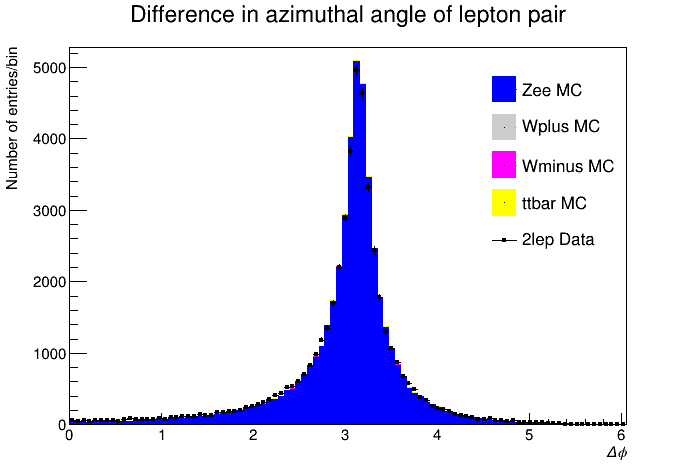
\includegraphics[width=\linewidth]{plots/25-02-2021/Zee-Stack-delta phi_(inv--mass-cut-lower-60GeV_2lep=ee)_25-02-21_09-30.png}
        (A)
    \end{minipage}\hfill
    \begin{minipage}{0.5\textwidth}
        \centering
        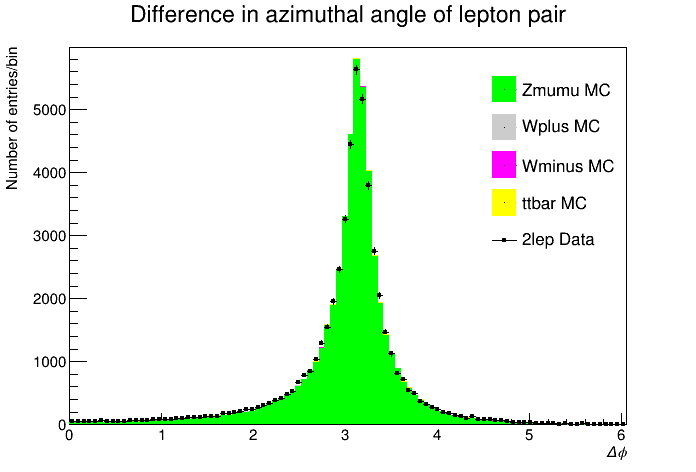
\includegraphics[width=\linewidth]{plots/25-02-2021/Zmumu-Stack-delta phi_(inv--mass-cut-lower-60GeV_2lep=mumu)_25-02-21_09-40.png}
        (B)
    \end{minipage}
    \caption{(A) (B).  Cuts: }
    \label{fig:}
\end{figure}

%%%%%%%%%%%%% 9:50 %%%%%%%%%%%%%
\subsubsection*{09:50}
Plotting the total transverse momentum ($p_T$) of two leptons of the same type and opposite charge being produced.


Cuts being used in Fig.\ref{fig:Zmumu-Stack_total-pt_(min-cut_2lep=ll)_25-02-21}
\begin{lstlisting}
    lepCut = "(" + "(lep_charge[0] != lep_charge[1]) && (lep_type[0] == 13 && lep_type[1] == 13) && lep_n==2" + ")"

    t.SetAlias("inv_mass_Zll","sqrt(2*lep_pt[0]*lep_pt[1]*(cosh(lep_eta[0]-lep_eta[1])-cos(lep_phi[0]-lep_phi[1])))")
    t.Draw("(lep_pt[0]+lep_pt[1]) >> h_lep_pt_total(200,0,500e3)", weighting + "*" + lepCut)
\end{lstlisting}

\begin{figure}[h!]
    \centering
    \begin{minipage}{0.5\textwidth}
        \centering
        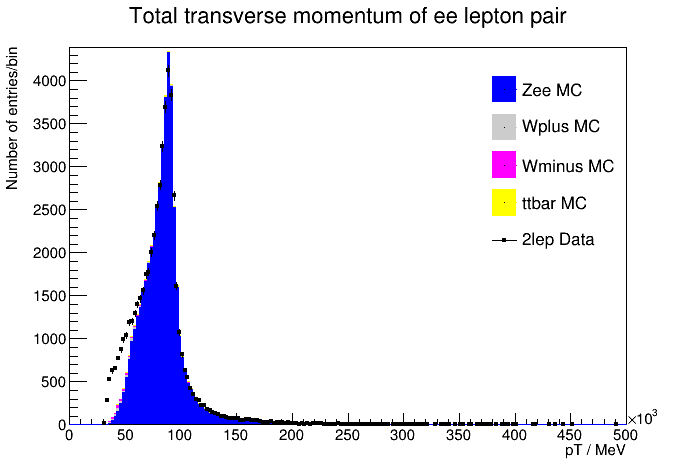
\includegraphics[width=\linewidth]{plots/25-02-2021/Zee-Stack_total-pt_(min-cut_2lep=e+e-)_25-02-21_09-50.png}
        (A)
    \end{minipage}\hfill
    \begin{minipage}{0.5\textwidth}
        \centering
        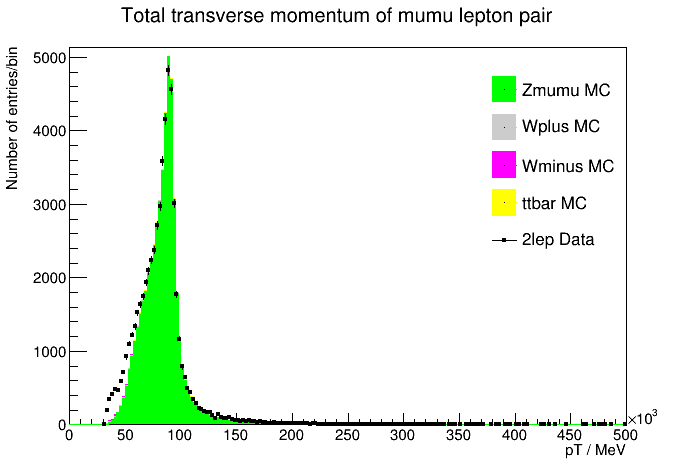
\includegraphics[width=\linewidth]{plots/25-02-2021/Zmumu-Stack_total-pt_(min-cut_2lep=mu+mu-)_25-02-21_09-50.png}
        (B)
    \end{minipage}
    \caption{(A) Total transverse momentum of e+e- pair. (B) Total transverse momentum of mu+mu- pair. Min cuts only: $lep_n==2$, opposite charge, specific type (e=11, mu=13)}
    \label{fig:Zmumu-Stack_total-pt_(min-cut_2lep=ll)_25-02-21}
\end{figure}

Cuts being used in Fig.\ref{fig:Zll-Stack_total-pt_(inv-mass-lower=60GeV_2lep=ll)_25-02-21}
\begin{lstlisting}
    lepCut = "(" + "(lep_charge[0] != lep_charge[1]) && (lep_type[0] == 13 && lep_type[1] == 13) && lep_n==2 && (inv_mass_Zll > 60000)" + ")"

    t.SetAlias("inv_mass_Zll","sqrt(2*lep_pt[0]*lep_pt[1]*(cosh(lep_eta[0]-lep_eta[1])-cos(lep_phi[0]-lep_phi[1])))")
    t.Draw("(lep_pt[0]+lep_pt[1]) >> h_lep_pt_total(200,0,500e3)", weighting + "*" + lepCut)
\end{lstlisting}

\begin{figure}[h!]
    \centering
    \begin{minipage}{0.5\textwidth}
        \centering
        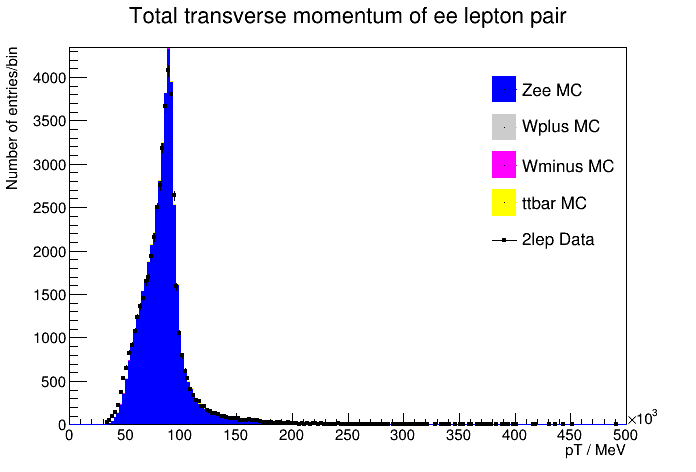
\includegraphics[width=\linewidth]{plots/25-02-2021/Zee-Stack_total-pt_(inv-mass-lower=60GeV_2lep=e+e-)_25-02-21_09-50.png}
        (A)
    \end{minipage}\hfill
    \begin{minipage}{0.5\textwidth}
        \centering
        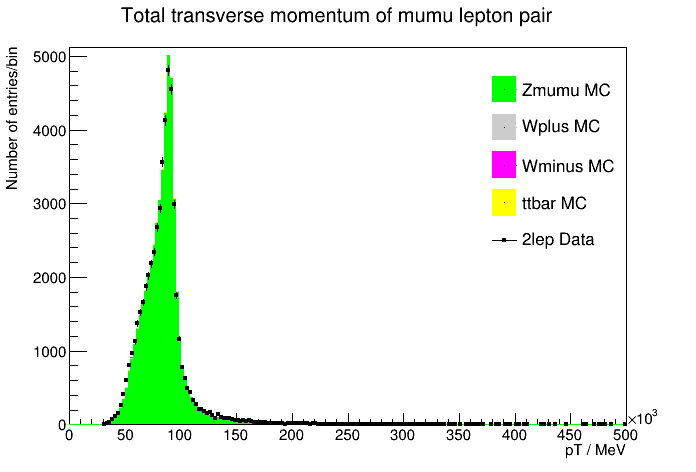
\includegraphics[width=\linewidth]{plots/25-02-2021/Zmumu-Stack_total-pt_(inv-mass-lower=60GeV_2lep=mu+mu-)_25-02-21_09-50.png}
        (B)
    \end{minipage}
    \caption{(A) Total transverse momentum of e+e- pair. (B) Total transverse momentum of mu+mu- pair. Only lower bound on invariant mass: $lep_n==2$, opposite charge, specific type (e=11, mu=13), and $m_{ll} > 60 GeV$ }
    \label{fig:Zll-Stack_total-pt_(inv-mass-lower=60GeV_2lep=ll)_25-02-21}
\end{figure}

%%%%%%%%%%%%% 9:50 %%%%%%%%%%%%%
\subsubsection*{09:50}
Plot the ptcone30.

Cuts for Fig.\ref{fig:Zll-stack_total-ptcone30_(min-cuts_2lep=ll)_25_02_21}
\begin{lstlisting}
# e=11, mu=13
lepCut = "(lep_charge[0] != lep_charge[1]) && (lep_type[0]==11 && lep_type[1]==11) && lep_n==2"

t.Draw("lep_ptcone30[0]+lep_ptcone30[1] >> h_lep_ptcone30(300,1e3,15e3)", weighting + "*" + lepCut)
\end{lstlisting}
\begin{figure}[h!]
    \centering
    \begin{minipage}{0.5\textwidth}
        \centering
        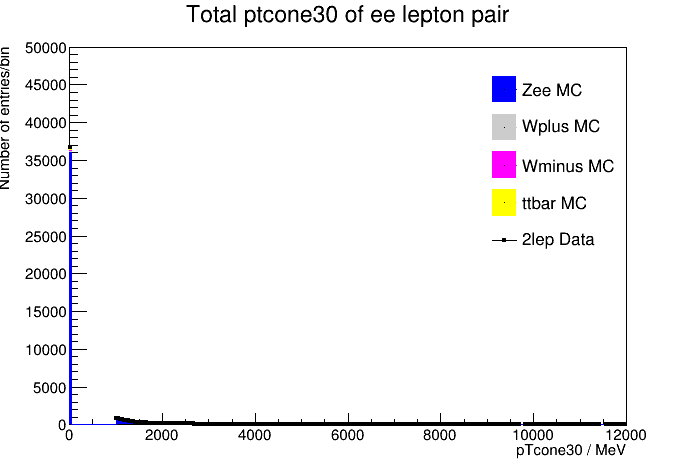
\includegraphics[width=\linewidth]{plots/25-02-2021/Zee-stack_total-ptcone30_(min-cuts_2lep=ee)_25_02_21_10-30_10-36.png}
        (A)
    \end{minipage}\hfill
    \begin{minipage}{0.5\textwidth}
        \centering
        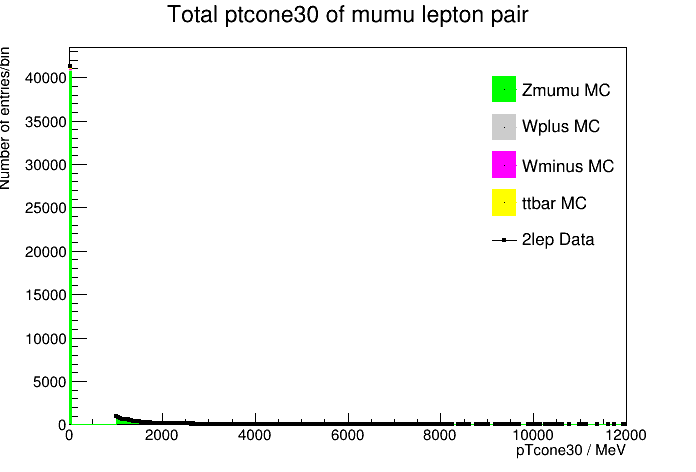
\includegraphics[width=\linewidth]{plots/25-02-2021/Zmumu-stack_total-ptcone30_(min-cuts_2lep=mumu)_25_02_21_10-30).png}
        (B)
    \end{minipage}
    \caption{(A) Total ptcone20 of ee pair. (B) Total ptcone20 of mumu pair.  Basic cuts: lep-n==2, same type, opposite charge.}
    \label{fig:Zll-stack_total-ptcone30_(min-cuts_2lep=ll)_25_02_21}
\end{figure}

Same as Fig.\ref{fig:Zll-stack_total-ptcone30_(min-cuts_2lep=ll)_25_02_21}, but different ptcone range to focus on $>$ 1 GeV. 
\\
Cuts for Fig.\ref{fig:Zmumu_Stack_total-ptcone30_(min-cuts_2lep=mumu)_25-02-21}
\begin{lstlisting}
    lepCut = "(lep_charge[0] != lep_charge[1]) && (lep_type[0]==11 && lep_type[1]==11) && lep_n==2"
    t.Draw("lep_ptcone30[0]+lep_ptcone30[1] >> h_lep_ptcone30(300,1e3,15e3)", weighting + "*" + lepCut)
\end{lstlisting}
\begin{figure}[h!]
    \centering
    \begin{minipage}{0.5\textwidth}
        \centering
        \includegraphics[width=\linewidth]{plots/}
        (A)
    \end{minipage}\hfill
    \begin{minipage}{0.5\textwidth}
        \centering
        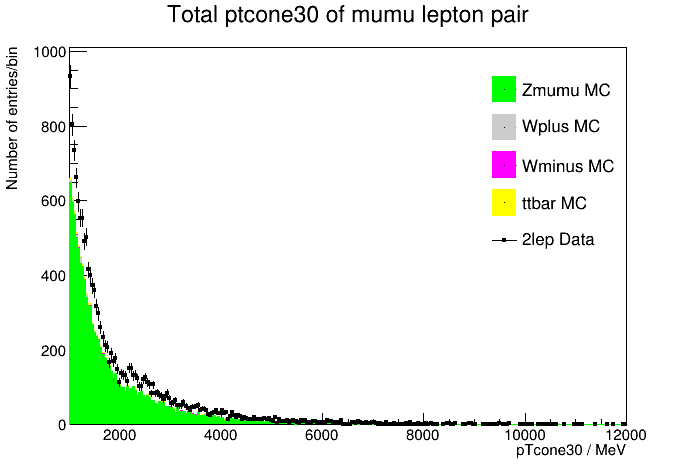
\includegraphics[width=\linewidth]{plots/25-02-2021/Zmumu_Stack_total-ptcone30_(min-cuts_2lep=mumu)_25-02-21_10-30.png}
        (B)
    \end{minipage}
    \caption{(A) Total ptcone20 of ee pair. (B) Total ptcone20 of mumu pair.  Basic cuts to include invariant mass: lep-n==2, same type, opposite charge, }
    \label{fig:Zmumu_Stack_total-ptcone30_(min-cuts_2lep=mumu)_25-02-21}
\end{figure}


Now applying invariant mass cut of lower bound of $>60 GeV$
Cuts for Fig.\ref{fig:Zee-stack_total-ptcone30_(inv-mass-lower=60GeV,2lep=ee)_25_02_21_10}
\begin{lstlisting}

\end{lstlisting}
\begin{figure}[h!]
    \centering
    \begin{minipage}{0.5\textwidth}
        \centering
        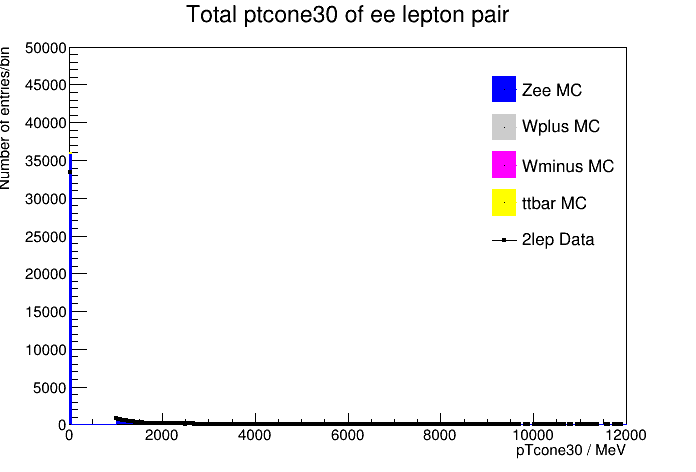
\includegraphics[width=\linewidth]{plots/25-02-2021/Zee-stack_total-ptcone30_(inv-mass-lower=60GeV,2lep=ee)_25_02_21_10-38).png}
        (A)
    \end{minipage}\hfill
    \begin{minipage}{0.5\textwidth}
        \centering
        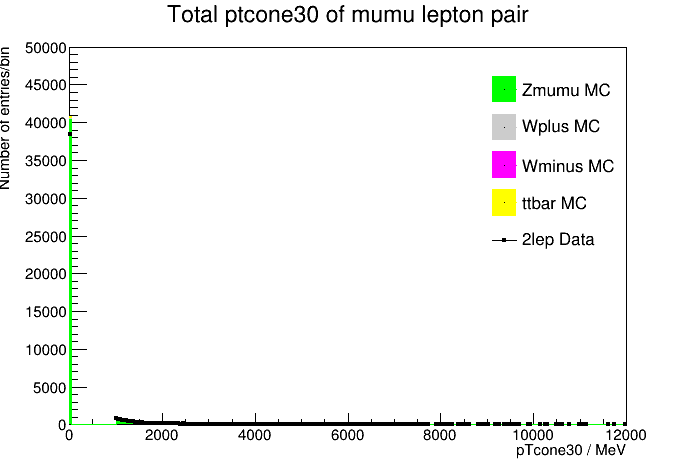
\includegraphics[width=\linewidth]{plots/25-02-2021/Zmumu-stack_total-ptcone30_(inv-mass-lower=60GeV,2lep=mumu)_25_02_21_10-30).png}
        (B)
    \end{minipage}
    \caption{(A) Total ptcone30 of ee pair being produced. (B) Total ptcone30 of mumu pair being produced. Cuts to include lower bound of invariant mass: lep-n==2, same type with opposite charge, invar-mass $>$ 60 GeV.}
    \label{fig:Zee-stack_total-ptcone30_(inv-mass-lower=60GeV,2lep=ee)_25_02_21_10}
\end{figure}



%%%%%%%%%%%%% 11:05 %%%%%%%%%%%%%
\subsubsection*{11:05}
Plot the etcone20.

Plotting the total ptcone20 with only the basic cuts. (same type opposite charge pair).  Fig.\ref{fig:Zll-stack_total-etcone_(min-cuts_2lep=l+l-)_25-02-21} as the cuts:
\begin{align}
# e=11, mu=13
lepCut ="(" + "(lep_charge[0] != lep_charge[1]) && (lep_type[0]== 13 && lep_type[1] == 13) && lep_n==2" + ")"    
    
t.SetAlias("inv_mass_Zll","sqrt(2*lep_pt[0]*lep_pt[1]*(cosh(lep_eta[0]-lep_eta[1])-cos(lep_phi[0]-lep_phi[1])))")
t.Draw("(lep_etcone20[0] + lep_etcone20[1]) >> h_lep_etcone20(200,-7e3,10e3)", weighting + "*" + lepCut)
\end{align}

\begin{figure}[h!]
    \centering
    \begin{minipage}{0.5\textwidth}
        \centering
        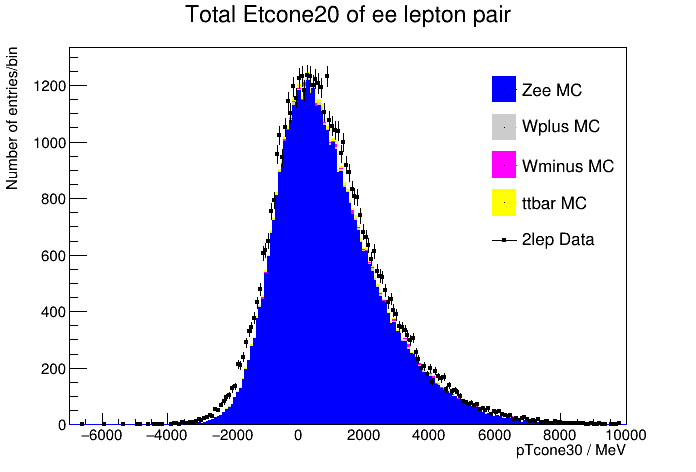
\includegraphics[width=\linewidth]{plots/25-02-2021/Zee-stack_total-etcone_(min-cuts_2lep=e+e-)_25-02-21_11-20.png}
        (A)
    \end{minipage}\hfill
    \begin{minipage}{0.5\textwidth}
        \centering
        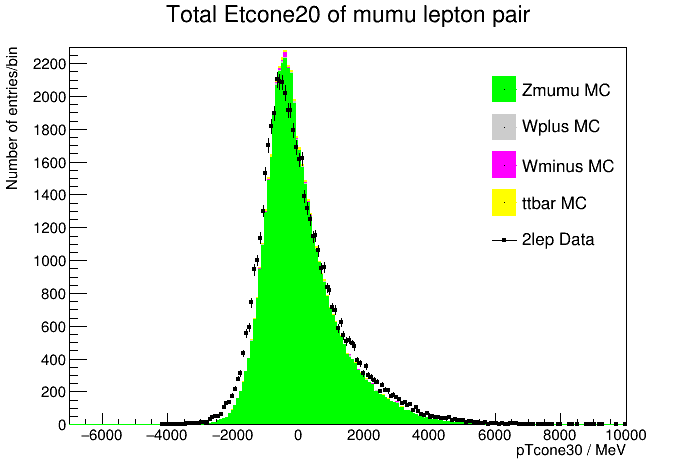
\includegraphics[width=\linewidth]{plots/25-02-2021/Zmumu-stack_total-etcone_(min-cuts_2lep=mu+mu-)_25-02-21_11-20.png}
        (B)
    \end{minipage}
    \caption{(A) Total etcone20 of ee pair produced (B) Total etcone20 of mumu pair produced. Basic Cuts: same type, opposite charged pair of leptons.}
    \label{fig:Zll-stack_total-etcone_(min-cuts_2lep=l+l-)_25-02-21}
\end{figure}



Applying the basic cuts along with the lower bound on the invariant mass ($m_{ll} > 60$ GeV).  Fig.\ref{} has the cuts:
\begin{lstlisting}
lepCut ="(" + "(lep_charge[0] != lep_charge[1]) && (lep_type[0]== 13 && lep_type[1] == 13) && lep_n==2 && inv_mass_Zll>60e3" + ")"    
    
    
    t.SetAlias("inv_mass_Zll","sqrt(2*lep_pt[0]*lep_pt[1]*(cosh(lep_eta[0]-lep_eta[1])-cos(lep_phi[0]-lep_phi[1])))")
    t.Draw("(lep_etcone20[0] + lep_etcone20[1]) >> h_lep_etcone20(200,-7e3,10e3)", weighting + "*" + lepCut)
\end{lstlisting}

\begin{figure}[h!]
    \centering
    \begin{minipage}{0.5\textwidth}
        \centering
        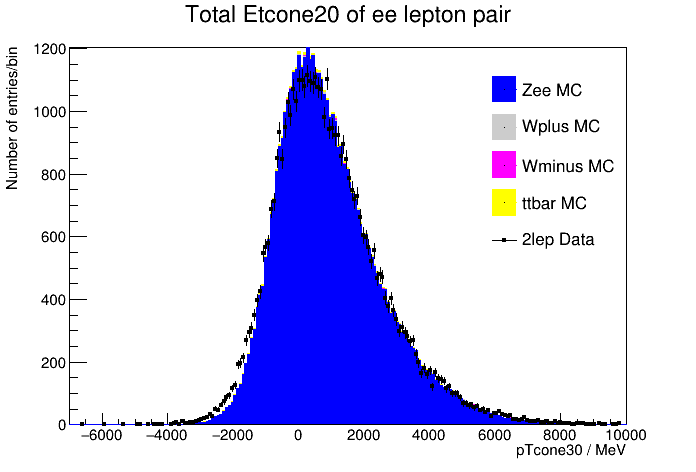
\includegraphics[width=\linewidth]{plots/25-02-2021/Zee-stack_total-etcone_(inv-mass-lower=60GeV_2lep=e+e-)_25-02-21_11-20.png}
        (A)
    \end{minipage}\hfill
    \begin{minipage}{0.5\textwidth}
        \centering
        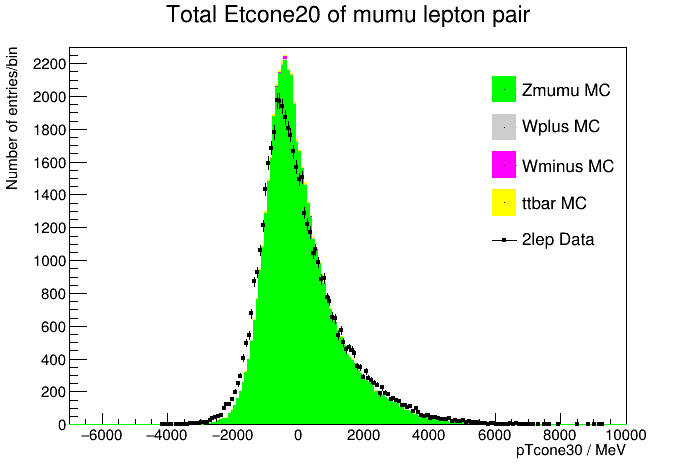
\includegraphics[width=\linewidth]{plots/25-02-2021/Zmumu-stack_total-etcone_(inv-mass-lower=60GeV_2lep=mu+mu-)_25-02-21_11-20).png}
        (B)
    \end{minipage}
    \caption{(A) Total etcone20 of ee pair produced (B) Total etcone20 of mumu pair produced. Cuts: invariant-mass $>$ 60 GeV, same type, opposite charged pair.}
    \label{fig:}
\end{figure}


%%%%%%%%%%%%% 11:30 %%%%%%%%%%%%% - Calculating the Zmumu cross section
\subsubsection*{11:30 - Lead BG - Calculating $\sigma(pp \rightarrow Z \rightarrow \mu\mu)$}
Calculating cross sections with varying cuts.
\\
The cross section: $\sigma (pp \rightarrow Z \rightarrow ee)$ is given by:
\begin{align}
    \sigma &= \frac{N^{selected} - N^{background}}{\epsilon \int L dt}
\end{align}
where
\begin{align}
     \epsilon &= \frac{\sum \text{weights for all MC events which pass selection cuts}}{\sum \text{weights for all events for that process}} 
\end{align}
\\
To start, calculate the cross section of $Z \rightarrow \mu\mu$ with cuts of:
\begin{itemize}
    \item $m_{ll} > 60$ GeV (lower bound on invaraint mass)
    \item Same lepton type 
    \item $lep_n == 2$ (number of leptons = 2)
    \item Opposite charge
\end{itemize}
Cross sections:
\begin{lstlisting}
t.SetAlias("inv_mass_Zll","sqrt(2*lep_pt[0]*lep_pt[1]*(cosh(lep_eta[0]-lep_eta[1])-cos(lep_phi[0]-lep_phi[1])))")
    
lepCut ="(" + "(lep_charge[0] != lep_charge[1]) && (lep_type[0]== 13 && lep_type[1] == 13) && lep_n==2 && inv_mass_Zll > 60e3" + ")"    
  
t.Draw("lep_n >> h_lep_n(3,-0.5,3.5)", weighting + "*" + lepCut)
\end{lstlisting}

Data sources: 
\begin{itemize}
    \item Background
    \subitem Wminus\_2lep, Wplus\_2lep, ttbar\_lep
    \item Source
    \subitem 2lep
    \item MC 
    \subitem Zmumu
\end{itemize}

\begin{align}
    N^{selected} &= 5288466
    \\
    N^{background}_{Wminus_2lep} &= 5904
    \\
    N^{background}_{Wplus_2lep} &= 6876
    \\
    N^{background}_{ttbar_lep} &= 3.063e4
    \\
    \epsilon &= \frac{5.153e6}{19631161.45} %3.063
\end{align}
Results:
\begin{align}
    \epsilon &= 0.2624908369850934
    \\
    \sigma (pp \rightarrow Z \rightarrow \mu\mu) &=  1.985479254338143e-09
\end{align}


%%%%%%%%%%%%% 12:12 %%%%%%%%%%%%% - Re-calculate the Zee cross section
\subsubsection*{12:12 - Calculating $\sigma(pp \rightarrow Z \rightarrow ee)$}
Data sources: 
\begin{itemize}
    \item Background
    \subitem Wminus\_2lep, Wplus\_2lep, ttbar\_lep
    \item Source
    \subitem 2lep
    \item MC 
    \subitem Zee
\end{itemize}

Cuts:
\begin{lstlisting}
t.SetAlias("inv_mass_Zll","sqrt(2*lep_pt[0]*lep_pt[1]*(cosh(lep_eta[0]-lep_eta[1])-cos(lep_phi[0]-lep_phi[1])))")
    
lepCut ="(" + "(lep_charge[0] != lep_charge[1]) && (lep_type[0]== 11 && lep_type[1] == 11) && lep_n==2 && inv_mass_Zll > 60e3" + ")"    
  
t.Draw("lep_n >> h_lep_n(3,-0.5,3.5)", weighting + "*" + lepCut)
\end{lstlisting}

Integral values
\begin{align}
    N^{selected} &= 4932622
    \\
    N^{background}_{Wminus_2lep} &= 6173
    \\
    N^{background}_{Wplus_2lep} &= 7268
    \\
    N^{background}_{ttbar_lep} &= 3.783e4
    \\
    \epsilon &= \frac{4.633e6}{19630128.89}
\end{align}

Results:
\begin{align}
    \epsilon &= 0.23601475191332785
    \\
    \sigma (pp \rightarrow Z \rightarrow ee) &= 2.0550872277842785e-09 b
\end{align}



%%%%%%%%%%%%% 14:00 %%%%%%%%%%%%% - Investigating Effect of transverse momentum lower bound cut on the cross section. 
\subsubsection*{14:00 - Lead BG}
Plot the total pt on a log y-scale to select a lower bound cut cut 

Cuts being used on Fig.\ref{fig:}

\begin{lstlisting}
# e=11, mu=13
lepCut = "(" + "(lep_charge[0] != lep_charge[1]) && (lep_type[0] == 11 && lep_type[1] == 11) && lep_n==2 && (inv_mass_Zll > 60e3)" + ")"

t.SetAlias("inv_mass_Zll","sqrt(2*lep_pt[0]*lep_pt[1]*(cosh(lep_eta[0]-lep_eta[1])-cos(lep_phi[0]-lep_phi[1])))")

t.Draw("(lep_pt[0]+lep_pt[1]) >> h_lep_pt_total(200,0,500e3)", weighting + "*" + lepCut)
\end{lstlisting}

\begin{figure}[h!]
    \centering
    \begin{minipage}{0.5\textwidth}
        \centering
        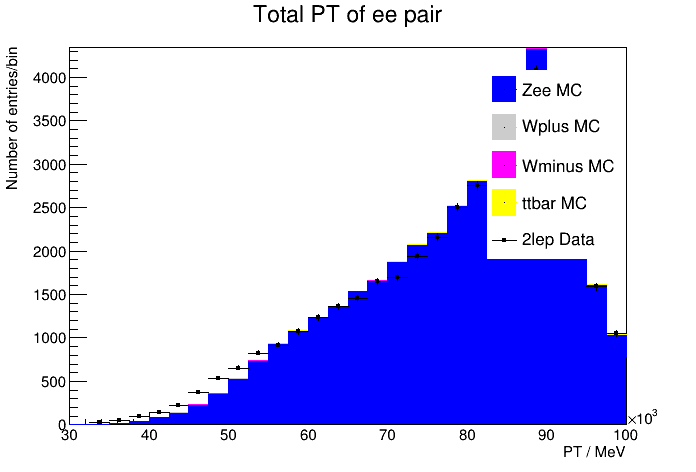
\includegraphics[width=\linewidth]{plots/25-02-2021/Zee-stack-(invar-mass-lower=60GeV,2lep=e+e-)-totalPt-lower-bound-justification_25-02-21_15-04.png}
        (A)
    \end{minipage}\hfill
    \begin{minipage}{0.5\textwidth}
        \centering
        \includegraphics[width=\linewidth]{plots/}
        (B)
    \end{minipage}
    \caption{(A) Total transverse momentum of electron pair (B) Total transverse momentum of muon pair. Cuts: }
    \label{fig:Zee-stack-(invar-mass-lower=60GeV,2lep=e+e-)-totalPt-lower-bound-justification_25-02-21}
\end{figure}

From Fig.\ref{fig:Zee-stack-(invar-mass-lower=60GeV,2lep=e+e-)-totalPt-lower-bound-justification_25-02-21}, choose a lower bound on PT of $55 GeV$.


%%%%%%%%%%%%% 15:00 %%%%%%%%%%%%% - Investigating Effect of transverse momentum lower bound cut on the cross section. 
\subsubsection*{15:00 - Calculating $\sigma(pp \rightarrow Z \rightarrow ee)$ lower cut on PT}
Calculating the cross section of... with the cuts :

\begin{lstlisting}
lepCut = "(" + "(lep_charge[0] != lep_charge[1]) && (lep_type[0] == 11 && lep_type[1] == 11) && lep_n==2 && (inv_mass_Zll > 60e3)" + ")"

t.SetAlias("inv_mass_Zll","sqrt(2*lep_pt[0]*lep_pt[1]*(cosh(lep_eta[0]-lep_eta[1])-cos(lep_phi[0]-lep_phi[1])))")

t.Draw("(lep_pt[0]+lep_pt[1]) >> h_lep_pt_total(200, 55e3,500e3)", weighting + "*" + lepCut)
\end{lstlisting}

Integral values
\begin{align}
    N^{selected} &= 4.66e6
    \\
    N^{background}_{Wminus\_2lep} &= 3006
    \\
    N^{background}_{Wplus\_2lep} &= 3256
    \\
    N^{background}_{ttbar\_lep} &= 3.687e4
    \\
    \epsilon &= \frac{4.472e6}{19630128.89}
\end{align}

Results:
\begin{align}
    \epsilon &= 0.2278130737225129
    \\
    \sigma (pp \rightarrow Z \rightarrow ee) &= 2.0137158391152733e-09 b
\end{align}


%%%%%%%%%%%%% 15:35 %%%%%%%%%%%%% - Investigating Effect of transverse momentum lower bound cut on Z->mumu cross section. 
\subsubsection*{15:35 - Calculating $\sigma(pp \rightarrow Z \rightarrow \mu\mu)$ lower cut on PT = 55 GeV}

\begin{lstlisting}
lepCut = "(" + "(lep_charge[0] != lep_charge[1]) && (lep_type[0] == 13 && lep_type[1] == 13) && lep_n==2 && (inv_mass_Zll > 60e3)" + ")"

t.SetAlias("inv_mass_Zll","sqrt(2*lep_pt[0]*lep_pt[1]*(cosh(lep_eta[0]-lep_eta[1])-cos(lep_phi[0]-lep_phi[1])))")

t.Draw("(lep_pt[0]+lep_pt[1]) >> h_lep_pt_total(200, 55e3,500e3)", weighting + "*" + lepCut)
\end{lstlisting}

Integral values
\begin{align}
    N^{selected} &= 5.061e6
    \\
    N^{background}_{Wminus\_2lep} &= 3620
    \\
    N^{background}_{Wplus\_2lep} &= 4241
    \\
    N^{background}_{ttbar\_lep} &= 2.985e4
    \\
    \epsilon &= \frac{4.912e6}{19631161.45}
\end{align}

Results:
\begin{align}
    \epsilon &= 0.25021443649733727
    \\
    \sigma (pp \rightarrow Z \rightarrow \mu\mu) &= 1.9948267037420005e-09 b
\end{align}


%%%%%%%%%%%%% 16:05 %%%%%%%%%%%%% - Increase transverse momentum lower bound cut on Z->mumu cross section to 80 GeV. 
\subsubsection*{15:35 - Calculating $\sigma(pp \rightarrow Z \rightarrow \mu\mu)$ lower cut on PT = 80 GeV}

\begin{lstlisting}
lepCut = "(" + "(lep_charge[0] != lep_charge[1]) && (lep_type[0] == 13 && lep_type[1] == 13) && lep_n==2 && (inv_mass_Zll > 60e3)" + ")"

t.SetAlias("inv_mass_Zll","sqrt(2*lep_pt[0]*lep_pt[1]*(cosh(lep_eta[0]-lep_eta[1])-cos(lep_phi[0]-lep_phi[1])))")

t.Draw("(lep_pt[0]+lep_pt[1]) >> h_lep_pt_total(200, 80e3,500e3)", weighting + "*" + lepCut)
\end{lstlisting}

Integral values. 
\begin{align}
    2lep &= 3.264e6
    \\
    Wminus\_2lep &= 1719
    \\
    Wplus\_2lep &= 2138
    \\
    ttbar\_lep &= 2.485e4
    \\
    Zmumu &= 3.142e6
\end{align}


\begin{align}
    N^{selected} &= 3.264e6
    \\
    N^{background}_{Wminus\_2lep} &= 1719
    \\
    N^{background}_{Wplus\_2lep} &= 2138
    \\
    N^{background}_{ttbar\_lep} &= 2.485e4
    \\
    \epsilon &= \frac{3.142e6}{19631161.45}
\end{align}

Results:
\begin{align}
    \epsilon &= 0.16005166113082933
    \\
    \sigma (pp \rightarrow Z \rightarrow ee) &= 2.0085507247902045e-09
\end{align}


%%%%%%%%%%%%% 16:22 %%%%%%%%%%%%% - Increase transverse momentum lower bound cut on Z->ee cross section to 80 GeV. 
\subsubsection*{15:35 - Calculating $\sigma(pp \rightarrow Z \rightarrow ee)$ lower cut on PT = 80 GeV}


\begin{lstlisting}
lepCut = "(" + "(lep_charge[0] != lep_charge[1]) && (lep_type[0] == 11 && lep_type[1] == 11) && lep_n==2 && (inv_mass_Zll > 60e3)" + ")"

t.SetAlias("inv_mass_Zll","sqrt(2*lep_pt[0]*lep_pt[1]*(cosh(lep_eta[0]-lep_eta[1])-cos(lep_phi[0]-lep_phi[1])))")

t.Draw("(lep_pt[0]+lep_pt[1]) >> h_lep_pt_total(200, 80e3,500e3)", weighting + "*" + lepCut)
\end{lstlisting}

Integral values. 
\begin{align}
    2lep &= 2.983e6
    \\
    Wminus\_2lep &= 1110
    \\
    Wplus\_2lep &= 1170
    \\
    ttbar\_lep &= 3.101e4
    \\
    Zee &= 2.838e6
\end{align}


\begin{align}
    N^{selected} &= 2.983e6
    \\
    N^{background}_{Wminus\_2lep} &= 1110
    \\
    N^{background}_{Wplus\_2lep} &= 1170
    \\
    N^{background}_{ttbar\_lep} &= 3.101e4
    \\
    \epsilon &= \frac{2.838e6}{19630128.89}
\end{align}

Results:
\begin{align}
    \epsilon &= 0.1445736814008255
    \\
    \sigma (pp \rightarrow Z \rightarrow ee) &= 2.0273066850004195e-09
\end{align}

\begin{tabular}{ c | c | c }
  \hline			
  var. & val. & uncert. \\
  
  $N^{selected}$ & - & - \\
  
  $N^{background}_{Wminus\_2lep}$ & - & - \\
  
  $N^{background}_{Wplus\_2lep}$ & - & - \\
  
  $N^{background}_{ttbar\_lep}$ & - & - \\
  
  $\epsilon_{num}$ & - & - \\
  
  $\epsilon_{den}$ & - & - \\
  \hline  
\end{tabular}




TODO:
\\
 - Plot sigma for different cuts on same plot.

